% !TEX root =  manuscript.tex
\subsection{Computer Vision Techniques (RQ3)}


In order to investigate how computer vision is applied, we studied:
(1)~what visual artifacts are used, generated, or extracted from the software,
and (2)~what computer vision techniques are used to process or analyze the visual artifacts.
We recall that visual artifacts are visual data (e.g.,  images) used by one or more computer vision
techniques, with the final objectives of addressing a software engineering problem.


\begin{figure}
%    \revised{0.98\linewidth}{
    \centering
    %\fbox{
    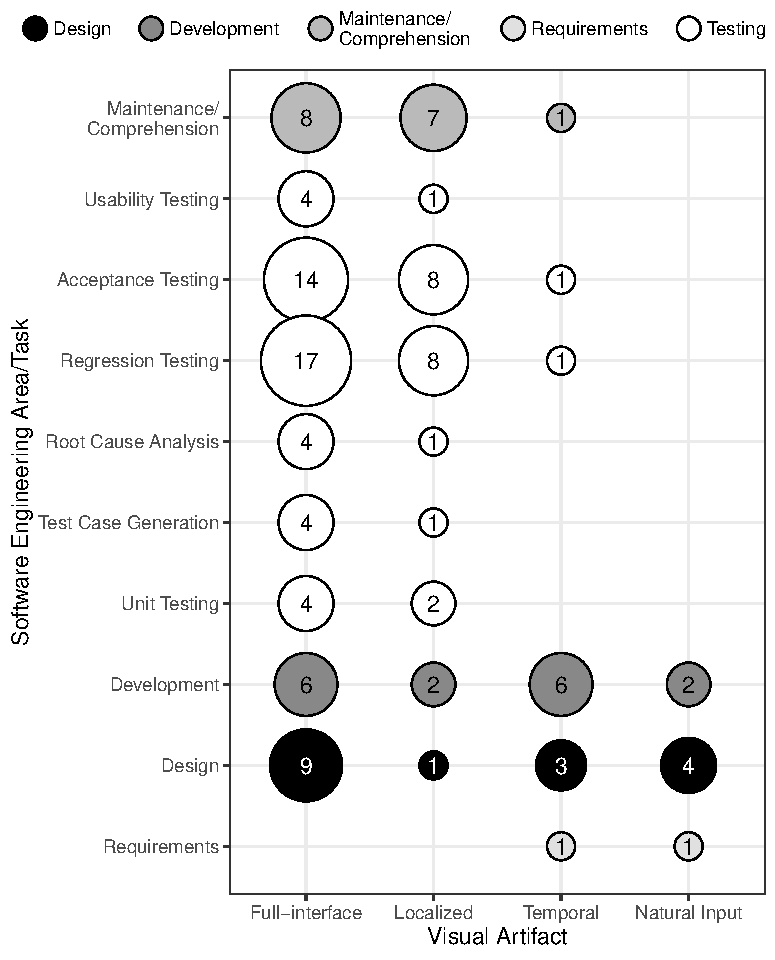
\includegraphics[width=0.8\linewidth]{survey/figures/visual-artifacts-bubble-plot}
    %}
    \caption{Distribution of visual artifacts per SE area \& task.}\label{fig-artifacts}
%    }
\end{figure}



\header{Artifact Categories}
Through our survey of the field, we classified the 
%identified a number of classes of 
visual artifacts used in the literature into four categories:
(1)~full-interface artifacts, (2)~localized artifacts,
(3)~temporal artifacts, and (4)~natural input artifacts. 
\Cref{fig-artifacts} shows the distribution of such visual artifacts 
with respect to the SE area/tasks.

The first category, \emph{full-interface visual artifacts}, typically represents
screenshots of the entire user interface of the system (whether a web browser or
desktop application, as well as other forms such as visual content of TVs and car displays)
~\cite{Choudhary-2010-ICSM,Delamaro-2011-STVR,
Choudhary-2012-ICST,Semenenko-2013-ICSM,Choudhary-2013-ICSE,Nguyen-2015-ASE,
Mahajan-2015-ICST,Deka-2016-UIST, Hori-2015-SEKE,Mahajan-2016-ICST,Feng-2016-ASE,
Patric-2016-ASE,Deka-2017-UIST,Wan-2017-STVR,He-2016-ICWS,Zhang-2017-ASE,Chen-2017-IUI,
Kirac-2018-JSS,Xu-2018-TOIT,Kuchta-2018-EMSE}.
This type of artifact simply has one large screenshot that captures the entire interface. 
This artifact has been used most commonly to capture the \textit{visual state} of the application
(regardless of the platform), and analyzed further to perform various forms of testing
(e.g., regression, acceptance, or test generation).

However, full-interface artifacts capture the visual state of the system at a coarse-grained
level of granularity, which renders them less applicable when a more detailed analysis is needed. This is because the full-interface 
captures the interface as a whole, and is therefore not very useful when the goal is more micro-scale, such as analyzing or recognizing a particular icon for instance. 
For these cases, our survey revealed another category containing  \emph{localized visual artifacts}.
In this case, visual artifacts are created at the level of a 
specific component, an area of interest, or a certain feature \cite{Chang-2010-CHI,
Alegroth-2013-ICST, Mahajan-2014-ASE, Amalfitano-2014-WISE, Selay-2014-DICTA,
Burg-2015-UIST, Leotta-2018-STVR, canvas_icst2018}.
Compared to full-interface visual artifacts, this type of artifact is more beneficial
for scenarios where analysis needs to be performed for a specific component or feature in a system. 
For instance, localized visual artifacts have been used to create a test case for a GUI
(by recording and tracking a single visual artifact for UI elements) \cite{Chang-2010-CHI},
or in debugging the rendering or capturing the behaviour of a specific HTML element in a web application~\cite{Burg-2015-UIST}. 
Had the record-and-playback used full-interface instead of localized visual artifacts, then the analysis wouldn't make much since because the test script operates at the level of elements, not entire interfaces. 

The third category that emerged is \emph{temporal artifacts}, in which the visual information
captures the \emph{dynamic behaviour} of some sequence or chain of information, states, or events
~\cite{Li-2010-CHI, Lin-2014-TSE,Ponzanelli-2016-ICSE,Bao-2017-EMSE}. 
For instance,~\citet{Bao-2017-EMSE} use a temporal artifact (a video screen recording) to construct a
tool to help researchers conducting user studies of developers' behaviours
to automatically distill and transcribe their actions, inputs, and event sequences
by capturing a video screen recording of their work session.

Finally, 
the last identified category is \emph{natural input artifacts}.
These artifacts capture a natural representation or interaction with a human user.
The only example of this artifact that we found in the collected literature are
hand-sketches~\cite{Scharf-2013-ICSE, Reiss-2018-ASEj}.
This type of artifact provides a number of benefits:
(1)~it provides a more intuitive and natural way for software engineers to interact with,
    design, develop, or test their software, and
(2)~it allows a broad degree of freedom in capturing user input,
    which can be useful when modelling or analyzing multi-variable complex systems.



% !TEX root =  manuscript.tex

%\begin{table*}[t!]
\begin{sidewaystable}
    \caption{Major computer vision algorithms used in the collected papers.}
    \centering
    %\renewcommand{\arraystretch}{1.2}
	\setlength{\tabcolsep}{9pt}
%	\revised{\textwidth}{
    \begin{tabular}{l l p{5.5cm} p{3cm}}
        \toprule
        \textbf{Visual Technique}	& \textbf{Algorithm}	& \textbf{Description}		& \textbf{Utilized in} \\
        \midrule
        \multirow{9}{*}{Differential} 	
        		& \multirow{2}{*}{Image diff}
        													& A processing method whose output is a function of the 
        														difference between a pair of input images (e.g. PID--Perceptual Image Differencing~\cite{ref:PID},
																PHash--Perceptual Hashing~\cite{ref:PHash}).
       	 		& \cite{Selay-2014-DICTA, Delamaro-2011-STVR, Deka-2016-UIST, Kuchta-2018-EMSE, Zhao-2019-ICSE,Liang-2013-UIST,Lim-2018-UIST,Bao-2015-ICSE,  Choudhary-2010-ICSM, Li-2010-CHI, Mahajan-2014-ASE, Burg-2015-UIST, Mahajan-2015-ICST, Ponzanelli-2016-ICSE, Mahajan-2016-ICST, Deka-2017-UIST, Bao-2017-EMSE, Chen-2017-IUI, Kirac-2018-JSS, Xu-2018-TOIT, Moran-ICSE-2018, Moran-2018-ASE}   \\
		& & & \\
        	 																				
                & \multirow{2}{*}{Probability distribution distance}
                                   							& Measuring the distance between \emph{distributions} of pixels 
                                   							in a pair of images (e.g. $\chi^2$ distribution distance). 
                & \cite{Choudhary-2010-ICSM, Choudhary-2012-ICST, Choudhary-2013-ICSE, Lin-2014-TSE,Hori-2015-SEKE, Feng-2016-ASE,He-2016-ICWS, Xu-2018-TOIT, bajammal2018generating, Moran-2018-ASE} \\
                                   							
		\midrule
        \multirow{8}{*}{Transformational}
        		& \multirow{2}{*}{Color/Spatial transformation}
        													& Applying a transformation matrix to the spatial or color-space of one or more images, or transforming spatial regions into abstract data.
				& \cite{Dixon-2010-CHI, Reiss-2018-ASEj,    Fails-2003-CHI, Zheng-2009-CHI,Givens-2013-ICSE,Bao-2015-ICSE,Reinecke-2016-CHI, Caetano-2002-AAAI, Coyette-2007-INTERACT, Dixon-2011-CHI, Seifert-2011-MobileHCI,  Natarajan-2018-MOBILESoft, Osman-2018-SEAA, Huang-2019-CHI, Li-2010-CHI, Patric-2016-ASE, Wan-2017-STVR, Kirac-2018-JSS, canvas_icst2018, Moran-TSE-2018, Moran-ICSE-2018, Xiao-2019-ICSE} \\

		& & & \\
                & \multirow{2}{*}{Optical character recognition}
                                    						& Recognizing images of strings and converting them 
                                    						into textual data.
                & 
%                \multirow{2}{*}{
                	\cite{Yu-2019-ASE, Chang-2010-CHI, Amalfitano-2014-WISE, Nguyen-2015-ASE, Ponzanelli-2016-ICSE, Bao-2018-TSE, Tanno-2018-ICSTW, Xiao-2019-ICSE}
%                } 
            \\
		\midrule				
            	& Template matching		& Finding where an image is located within another image. 
				& \cite{Alegroth-2013-ICST, Dixon-2010-CHI, Bao-2018-TSE, Givens-2013-ICSE, Yu-2019-ASE, Chang-2010-CHI, Semenenko-2013-ICSM, Lin-2014-TSE, Bao-2017-EMSE, Chen-2017-IUI, Leotta-2018-STVR, Stocco-2018-FSE, Tanno-2018-ICSTW} \\
		Search							&   &   &   \\
				& Machine learning		& Finding closest visual matches or categories based on learning patterns in visual data. 
				& \cite{Scharf-2013-ICSE,  Landay-2001-IEEEComputer,  Deka-2016-UIST, Zhang-2017-ASE, Reiss-2018-ASEj,       Wu-2017-CSCW,Chen-2018-ICSE,Sun-2018-ICML,Zhao-2019-ICSE,Swearngin-2019-CHI,Yuan-2020-CHI,Wu-2020-CHI,Fails-2003-CHI} \\
        \bottomrule
    \end{tabular}
		\label{tbl:cv-algorithms}
%	}
%\end{table*}
\end{sidewaystable}

\header{Visual Techniques Taxonomy}

\begin{figure}
    \centering
    %\fbox{
    
\includegraphics[width=\linewidth]{survey/figures/taxonomy}
    %}
    \caption{Synthesized taxonomy of visual techniques.}
    \label{fig:taxonomy-rq3}
\end{figure}

In this section, we describe a taxonomy of visual techniques.
The taxonomy was synthesized from the pool of papers we collected 
in this survey. 
This taxonomy has not been used elsewhere, since 
there are no existing surveys on the use of computer 
vision techniques in software engineering.
For each paper, we analyzed the text and 
noted down the computer vision algorithms utilized by the authors 
to solve the software engineering problem being tackled.
After conducting this process over all collected papers, 
we grouped the algorithms and identified three main patterns of algorithms,
which are then collected in a taxonomy.
We built the taxonomy in an iterative manner,
where a new taxonomy category is defined if a certain computer vision algorithm 
can not be classified under any of the existing categories.

\autoref{fig:taxonomy-rq3} shows the resulting taxonomy.
As shown in the figure, we identified three main categories
of visual techniques used in software engineering research:
(1)~differential, (2)~transformational, and (3)~search techniques.
Each technique has sub-categories of algorithms, which will be described in Section \ref{sec:CV-algos}.


\emph{Differential techniques}: a visual analysis process that takes  two or more visual artifacts as input, and outputs their differences~\cite{Delamaro-2011-STVR,Choudhary-2012-ICST,
Choudhary-2010-ICSM,Alegroth-2013-ICST,Choudhary-2013-ICSE,Lin-2014-TSE,Mahajan-2014-ASE,
Amalfitano-2014-WISE,Selay-2014-DICTA,Burg-2015-UIST,Mahajan-2015-ICST,Hori-2015-SEKE,
Mahajan-2016-ICST,Feng-2016-ASE,Deka-2017-UIST,He-2016-ICWS,Kirac-2018-JSS,Xu-2018-TOIT}. 
The nature of these differences is typically case-specific and often targets a specific
feature that the paper is considering.
Differential techniques are commonly used in situations where a comparison of different aspects,
options, or versions of the software is desired.
For instance, they have been widely utilized for cross-browser testing
~\cite{Xu-2018-TOIT, Choudhary-2010-ICSM, He-2016-ICWS, Choudhary-2012-ICST, Selay-2014-DICTA},
where the goal is to check for any differences between two or more browsers in the way they 
render a web app.

The second category, \emph{transformational techniques}, achieve a specific software engineering task
by transforming the visual artifact into a more abstract type of information
~\cite{Scharf-2013-ICSE,Semenenko-2013-ICSM,Nguyen-2015-ASE,Deka-2016-UIST,Ponzanelli-2016-ICSE,
Patric-2016-ASE,Wan-2017-STVR,Bao-2017-EMSE,Zhang-2017-ASE,Reiss-2018-ASEj,canvas_icst2018,Kuchta-2018-EMSE}.
This transformation is typically case-specific, as the higher-level abstract information
is used to solve the specific instance of problems addressed in the paper.
For instance, this approach has been used to allow manual hand-drawn strokes as a method to specify
test executions and requirements~\cite{Scharf-2013-ICSE},
where transformational techniques are applied on hand-drawn stroke instances to extract testing
instructions and assertions from the strokes, and finally generate a working test case.

Finally, the third category is \emph{search techniques}~\cite{Chang-2010-CHI, Li-2010-CHI,Chen-2017-IUI,Leotta-2018-STVR}.
In this case, a visual artifact is used as a key to find information within a larger set of visual artifacts.
A popular example of this approach is visual record-and-playback tools such as Sikuli~\cite{Chang-2010-CHI}.
These tools first record component visual artifacts for every GUI element clicked or interacted with
by a developer or user, and then, in the playback phase, a visual search method is employed to locate
the element on screen to perform the recorded action (e.g., click).

\begin{figure}
%    \revised{\linewidth}{
    \centering
    %\fbox{
    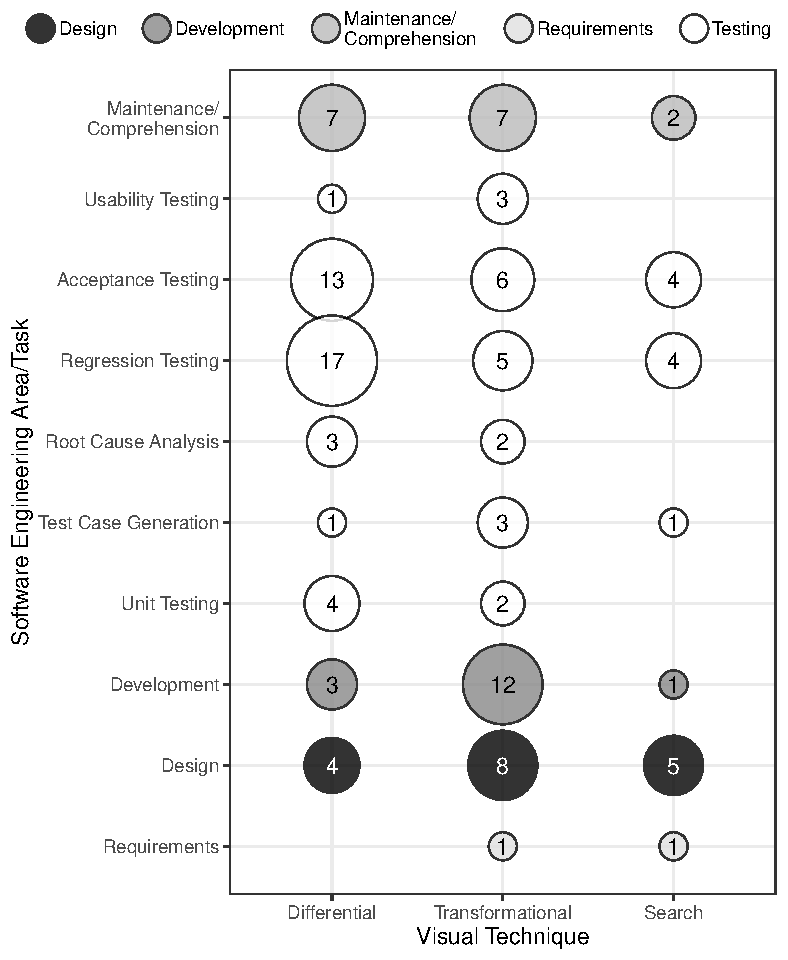
\includegraphics[width=0.8\linewidth]{survey/figures/bubbleplot-rq3}
    %}
    \caption{Distribution of visual techniques per SE area \& task.}\label{fig:bubbleplot-rq3}
%    }
\end{figure}


In order to have a better insight on the use of different 
categories of visual techniques,
the bubble plot of \autoref{fig:bubbleplot-rq3} shows their distribution over the various SE areas.
In the plot, software testing has a finer-grained granularity
since it is by far the most represented area in our final pool of papers.
We make a number of observations from the plot.
First, we notice that transformational techniques are more uniformly represented across all SE areas and tasks.
This is a somewhat expected result 
since transformational techniques are generic enough to be used 
on their own, or in addition to other techniques as pre- or post-processing steps. 
Next, we also notice that differential techniques were relatively common in testing tasks.
For instance, regression and acceptance testing greatly benefit from differential techniques,
since they are very well aligned towards detecting differences and therefore suitable for indicating regression faults.

    
\subsubsection{Computer Vision Algorithms}
\label{sec:CV-algos}

In addition to the preceding analysis of the high-level categories of visual techniques,
we also examine the specific computer vision algorithms used in the collected pool of papers.
\autoref{tbl:cv-algorithms} shows the algorithms that have emerged from our analysis.
We now describe each of the identified algorithms.

\header{Image Diff}
In these CV algorithms,
a pair of images is taken as input
and the output is defined as a function of the \emph{difference}  between the pair.
Various instances of these algorithms differ in their choice of the output function.
For instance, the most common variation uses the raw absolute difference as the output value~\cite{Choudhary-2010-ICSM,Li-2010-CHI,Mahajan-2014-ASE,Ponzanelli-2016-ICSE,
Deka-2017-UIST,Bao-2017-EMSE,Chen-2017-IUI,Kirac-2018-JSS,Moran-ICSE-2018},
where it is useful for faithfully detecting any \textit{pixel-level} difference.
Another variation adopts a more relaxed approach
where the output function captures only \emph{perceivable} differences by humans
using algorithms such as PID (Perceptual Image Differencing)~\cite{ref:PID},
PHash (Perceptual Hashing)~\cite{ref:PHash},
and Structural Similarity Index (SSIM)~\cite{ref:SSIM},
which aim to reduce false positives by mimicking human perception.
These techniques were utilized in~\cite{Mahajan-2015-ICST,Mahajan-2016-ICST,
Xu-2018-TOIT,Moran-ICSE-2018,Moran-2018-ASE,Burg-2015-UIST}. 

\header{Probability Distribution Distance}
These algorithms quantify distances in \emph{populations} of pixels,
as opposed to a pixel-wise comparison.
The goal here is to measure how similar two given distributions are,
such as image \emph{histograms}~\cite{223129} which give the distribution of pixels in an image.
This is then used to establish whether the two
distributions of pixels can be assumed to represent similar visual
information.
The $\chi^2$ histogram distance (for both coloured and grayscale data)
is by far the most commonly used distribution distance
in our pool of papers~\cite{Choudhary-2012-ICST,Choudhary-2013-ICSE,
Hori-2015-SEKE,Feng-2016-ASE,He-2016-ICWS, Moran-2018-ASE},
as it is readily available in many implementations
and provides a simple and effective approach for the needed quantification of distance.

\header{Color/Spatial Transformation}
These algorithms perform a transformation
of the spatial or color-space of one or more images~\cite{Li-2010-CHI,Patric-2016-ASE,Wan-2017-STVR,Kirac-2018-JSS,
canvas_icst2018,Moran-TSE-2018,Moran-ICSE-2018,Xiao-2019-ICSE}.
This constitutes applying a 2D or 3D transformation matrix
on the desired geometric space (e.g., a rearrangement of color-space).
This class of algorithms has been used in our pool of papers
to perform tasks such as extracting structure from images,
aligning images, and various forms of thresholding to extract content.

\header{Optical Character Recognition (OCR)}
OCR algorithms use a series of computer vision analyses
to recognize strings in images.
Once the string is recognized, another sequence of steps
converts each character in the image to textual data.
We found multiple papers in our pool (e.g., \cite{Chang-2010-CHI, Amalfitano-2014-WISE,
Nguyen-2015-ASE, Ponzanelli-2016-ICSE, Bao-2018-TSE, Tanno-2018-ICSTW, Xiao-2019-ICSE})
which have used OCR for tasks such as checking GUI component labels and
generating component labels from mockups/screenshots.

\header{Template Matching}
Another major class of CV algorithms used in the papers is template matching.
Here, one image is searched within another image or set of images.
That is, a visual scan is performed to find a template image (hence the name)
in a larger image or set of images.
Several papers in our pool~\cite{Chang-2010-CHI, Semenenko-2013-ICSM,
	Lin-2014-TSE, Bao-2017-EMSE, Chen-2017-IUI, Leotta-2018-STVR,
	Stocco-2018-FSE, Tanno-2018-ICSTW} have used this approach
to achieve tasks such as locating and finding coordinates of components and
checking the presence/absence of components or certain features within
a set of GUIs. While it may appear that template matching 
is related to the OCR class of techniques, it is actually different. 
This is because OCR converts an image to a string, while template matching finds the location of a given image within another image. 

\header{Machine Learning}
Machine learning has also been used by a few papers in our pool.
For instance, \emph{decision trees} were used for classifying web pages
in cross-browser testing~\cite{Choudhary-2012-ICST,Semenenko-2013-ICSM}.
\emph{Convolutional neural networks} (CNNs) were also used
to analyze GUIs and their content~\cite{Moran-TSE-2018,Semenenko-2013-ICSM}.
Furthermore, scale- and transformation-invariant features
(e.g.,  SURF--Speeded-Up Robust Features~\cite{ref:SURF}, Wavelets~\cite{ref:wavelet}),
which are basically features aiming at analyzing image structure and content,
were used to classify and detect GUI elements
~\cite{Xiao-2019-ICSE,Stocco-2018-FSE,Kuchta-2018-EMSE,Bao-2017-EMSE}.


% !TEX root =  manuscript.tex
\begin{table}%[t]
    \caption{Open-source and industrial computer vision tools and libraries utilized by papers in the pool. }
%     \andrea{This table was here in the previous revision as well. Highlight that the second part of the table are the industrial solutions the reviewer's asked for}}
    \centering
    %\small % bigger
    %\small %smaller
    \setlength{\tabcolsep}{8pt}
    \renewcommand{\arraystretch}{1.2}

%\revised{0.48\textwidth}{
    \begin{tabular}{p{2cm} p{6cm} p{3cm}}
    \toprule
    \textbf{Name} & \textbf{Scope} & \textbf{Utilized in} \\																
    \midrule
    
    OpenCV %~\cite{lib:opencv} 
            & provides data structures and algorithms for a wide variety of advanced computer vision processing 
            & \cite{Tanno-2018-ICSTW, Givens-2013-ICSE, Bao-2015-ICSE, Zhao-2019-ICSE, Moran-TSE-2018, Xiao-2019-ICSE,  Bao-2017-EMSE,   Feng-2016-ASE,  Stocco-2018-FSE, Mahajan-2016-ICST, Nguyen-2015-ASE, Leotta-2018-STVR, Mahajan-2015-ICST, Chang-2010-CHI,Choudhary-2010-ICSM, Choudhary-2012-ICST, Choudhary-2013-ICSE, Lin-2014-TSE} \\[0.5ex]
    Tesseract%~\cite{lib:abbyfinereader} 
            & extensible and modular open-source optical character recognition (OCR) engine
            & \cite{Nguyen-2015-ASE, Ponzanelli-2016-ICSE,Moran-TSE-2018,Yu-2019-ASE} \\[0.5ex]    
    FineReader%~\cite{lib:abbyfinereader} 
            & comprehensive OCR engine that includes relevant pre/post-processing steps and formats 
            & \cite{Bao-2018-TSE} \\[0.5ex]
    BoofCV%~\cite{lib:boofcv} 
            & performance-oriented library that focuses on real-time processing 
            & \cite{Ponzanelli-2016-ICSE} \\[0.5ex]
    ImageMagick%~\cite{lib:imagemagick} 
            & simple and easy to use tool and library for basic image transformations and analysis of color 
            & \cite{Mahajan-2014-ASE} \\[0.5ex]

    \midrule
    ITK (Insight ToolKit)%~\cite{lib:itk} 
    & specialized in image and coordinates matching, with comprehensive support for high-dimensional data & N/A \\[0.5ex]
    VLFeat%~\cite{lib:vlfeat} 
    & geared towards feature extraction, covering a large set of feature descriptors & N/A \\[0.5ex]
    ImageJ%~\cite{lib:imagej} 
    & a modular tool and library with an extensive number of plugins for various image analysis tasks & N/A \\[0.5ex]
    Amazon Rekognition, Google Vision AI, Azure CV
    %~\cite{lib:awscv, lib:googcv, lib:azurecv} 
    & cloud-based tools with a large number of pretrained analysis and recognition models & N/A \\[0.5ex]
    
    \bottomrule
    \end{tabular}
%    }
    \label{table:cvlibs}
    \end{table}



\header{Libraries and Tools}

% \revised{0.48\textwidth}{
\changed{
We also investigated what industrial or open-source 
libraries and tools were used by the papers in their 
implementation of computer vision techniques. 
\autoref{table:cvlibs} shows a list of the CV tools 
or libraries that have been used by the papers in our pool. 
The first column reports the name of the tool or library. 
The second column describes the scope of the library, 
and the last column shows the paper(s) that utilize 
a certain library to implement their CV analysis or processing. 
Papers that do not state which library or tool they used are not 
included in the table, and therefore the number of papers 
in the table is smaller than the total pool.
For the sake of completeness, we also included other 
CV tools and libraries that have not been used by 
any of the papers in our pool, which are marked 
by the ``N/A'' (not applicable) value in the last column. 
These tools were included in order to present the software 
engineering research community with an easy access to a list of 
other computer vision tools that they might find helpful to use. 
Due to the absence of queryable databases in 
which computer vision tools are listed, we resorted 
to manual search engine queries to find computer 
vision tools or libraries other than those already 
used by our pool. The queries we used were of the 
form ``alternative (libraries or tools) to X'', 
where X is one of the libraries already in our pool. %\andrea{vague}

The most commonly used library is \emph{OpenCV}.
\footnote{https://opencv.org} This library has 
implementations for a large number of CV algorithms, 
including all the algorithms we report in this 
survey (Section \ref{sec:CV-algos}). It was first 
released in 2000, and is still in active development. 
Other than OpenCV, a few other libraries were used 
by only a handful of papers. 
\emph{ImageMagick}\footnote{https://imagemagick.org/} 
is a simple and easy to use library offering basic 
quick image manipulations (e.g.,  resize, rotate).  
\emph{ImageJ}\footnote{https://imagej.net} is also 
quite similar in features and scope.
\emph{Tesseract}\footnote{https://github.com/tesseract-ocr/tesseract} 
is a popular open-source library that is modular and extensible, 
with support for more than 100 languages.
\emph{Abby FineReader}\footnote{https://abbyy.com/} is 
a commercial library that focuses specifically on 
OCR and includes many related preprocessing/postprocessing 
algorithms, as well as various file formats.
\emph{BoofCV}\footnote{http://boofcv.org} focuses 
on performance-tuned algorithms and is geared 
towards cases where real-time response is priority.
\emph{ITK}\footnote{https://itk.org/} focuses on 
high-dimensional visual data often present 
statistics and science, and also has extensive 
image coordinates matching algorithms that 
might be beneficial in a number of image 
matching applications. 
\emph{VLFeat}\footnote{https://vlfeat.org/} is 
geared towards implementing a wide variety of 
feature extraction and matching algorithms, 
enabling applications in image search or transformation.
Finally, there are cloud-based tools offered by 
major cloud hosting providers (e.g. Amazon Web 
Services, Google Cloud Platform, Microsoft Azure). 
The defining feature of these services is their 
cloud nature and the availability of many 
pre-trained computer vision models for various 
visual tasks, such as content tagging and 
visual path analysis. 
}

\begin{table}[]		\scriptsize
	\caption{Summary of the analysis approaches for the targeted research problems.}
	\begin{tabular}{lll}
		
		\textbf{Non-functional Property} & \textbf{Research Problems}                                                                        & \textbf{Approach}                                                                                                                                                                                                                                         \\
		\hline \\
		
		Accessibility           & \begin{tabular}[c]{@{}l@{}}- testing semantic roles\\ - repairing form labels\end{tabular} & \begin{tabular}[c]{p{4.5cm}}
			- identifying page regions, then computing and sorting ratios of visual locations, areas, visual size variance, and neural network classification. 
			\\ - abstracting form elements, then combining visual layout (relative spacing) with visual prominence (weight, size, color), and finally  optimizing label assignment
		\end{tabular} \\
		%		\begin{tabular}[c]{p{4.5cm}}Existing works perform syntax checks. Semantic roles and form labels are not tested or repaired. The work in this dissertation tests roles and repairs labels by analyzing visual cues from the page.\end{tabular} \\
		
		\\
		\hline \\
		
		Maintainability         & \begin{tabular}[c]{@{}l@{}}- generating reusable \\ components\end{tabular}                & 
		\begin{tabular}[c]{p{4.5cm}}- visual normalization of the page based on 
			element location, dimensions, and type, followed by histogram clustering \end{tabular} \\
		
		
		\\
		\hline \\
		
		Testability             & - testing canvas elements                                                                  & \begin{tabular}[c]{p{4.5cm}}- detecting and isolating object boundaries, then identifying their shapes, dimensions, colors, and hierarchy \end{tabular}                              \\
		
		
	\end{tabular}
	\label{tbl:summary-techniques}
\end{table}

\header{Overview of the proposed techniques}
In this dissertation, we propose a number of visual analysis techniques 
to improve the non-functional properties of testability, accessibility, and 
maintainability. An introduction to these properties and the motivation for 
exploring them is discussed in \Cref{chp:intro}. In \Cref{tbl:summary-techniques}, 
we show an overview of the approaches used, which are presented here only in a high-level and will be discussed in detail in their relevant chapters. 
While existing works are mostly based on using entire images, say, for diffing or searching, the techniques in this dissertation operate at a fine-grained level of analysis. By fine-grained we mean that the analysis focuses on very specific visual features that may potentially be helpful in addressing the research problem. 
For instance, when we analyze canvas elements, 
one fine-grained aspect that is used is extracting and identifying the boundaries 
of each object, in order to help detect the type of each object and express it in the 
DOM. Accordingly, the approaches are based on identifying what fine-grained features should be selected, where should they be collected from, how would they be combined,  
and how to analyze them to address the research problem. Each of these aspects 
is problem specific and need to be explored and determined according to the objective and constraints of the problem. 

\header{Summary}
The goal of this subsection was to explore what computer vision techniques
were used and what visual artifacts were extracted from the software.
To this end, we identified four categories of artifacts.
The first category, full-interface artifacts, represents cases
where the entire visual content of a software is used (e.g.,  entire desktop interface, entire console).
The second category is localized artifacts, where only a specific module
or component of the software is captured visually. 
Third, temporal artifacts capture the dynamic behavior of the states or events in a software. Finally, natural input artifacts capture natural forms of input by humans (e.g.,  hand sketches).
%
Visual artifacts are then processed by one or more of three visual techniques.
The first category, differential techniques, are based on various forms of contrasting two or more visual artifacts and using the differences to solve a software engineering problem.
The second category, transformational techniques, rely on transforming the visual artifact into a more abstract data structure on which further analysis can be conducted.
Finally, in search techniques, a visual artifact is used as a key to find information within a larger set of visual artifacts.

\autoref{tbl:cv-algorithms} shows the major computer vision algorithms used in the collected papers.
The visual technique column describes the high-level goal of what the algorithm is trying to achieve visually.
The algorithm column lists the specific algorithms that were used to achieve the task.
For instance, when papers wanted to do a differential examination of visual artifacts, the two computer vision approaches that were used were image diffing and distribution distances.

